\documentclass[11pt,letterpaper]{article}
\usepackage{graphicx, geometry, amsmath, natbib, booktabs, xcolor, listings}
\geometry{margin=1in}
\usepackage[colorlinks=true, linkcolor=black, citecolor=black, urlcolor=black, breaklinks=true]{hyperref}
\usepackage{url}
\urlstyle{same}
\Urlmuskip=0mu plus 1mu
\expandafter\def\expandafter\UrlBreaks\expandafter{\UrlBreaks\do\a\do\b\do\c\do\d\do\e\do\f\do\g\do\h\do\i\do\j\do\k\do\l\do\m\do\n\do\o\do\p\do\q\do\r\do\s\do\t\do\u\do\v\do\w\do\x\do\y\do\z\do\A\do\B\do\C\do\D\do\E\do\F\do\G\do\H\do\I\do\J\do\K\do\L\do\M\do\N\do\O\do\P\do\Q\do\R\do\S\do\T\do\U\do\V\do\W\do\X\do\Y\do\Z\do\0\do\1\do\2\do\3\do\4\do\5\do\6\do\7\do\8\do\9\do\/\do\-}%

\title{Reading Vector Patterns (RVP): A Cognitive-Inspired Approach to Near-Duplicate Short Text Detection}
\author{Anonymous}
\date{}

\begin{document}

\maketitle

\begin{abstract}
Near-duplicate detection for short text snippets is a critical task in information retrieval, content moderation, and question answering systems. Existing methods (MinHash LSH, edit distance, embedding-based approaches) struggle when text is too short for robust statistical features or when semantic similarity must be preserved despite lexical differences. This paper introduces Reading Vector Patterns (RVP), a novel cognitive-inspired approach that captures how text would be read by a human, not just what it contains. The method converts text to reading vectors---sequences of word-level cognitive load indicators (word length, word frequency, part-of-speech tags)---and compares these vectors using Dynamic Time Warping (DTW). We evaluate RVP against Jaccard n-gram, MinHash LSH, and Sentence-BERT baselines on the Quora Question Pairs dataset (10,000 question pairs, stratified split). Our experiments show that RVP achieves competitive ROC-AUC (0.695) with high recall (0.911) and processes pairs 6x faster than Sentence-BERT (11.1ms vs 67.8ms per pair). While Sentence-BERT achieves the highest F1-score (0.541), RVP provides an interpretable, training-free alternative that captures complementary signals through cognitive load patterns. Ablation studies reveal that word length is the most informative cognitive feature (F1=0.393), with frequency and POS tags providing marginal additional benefit. Our work opens a new direction for near-duplicate detection by incorporating cognitive processing patterns into text similarity measurement.
\end{abstract}

\section{Introduction}

\subsection{Problem Statement}

Near-duplicate detection is the task of identifying text pairs that convey the same meaning despite different wording, word order changes, or minor edits. This problem is particularly challenging for short text snippets (5-20 words), where traditional methods based on bag-of-words representations fail due to feature sparsity \cite{Broder1997}. Short text is prevalent in modern applications: question answering systems (Quora, Stack Overflow), search queries, social media posts, and chatbot conversations all involve short text snippets where near-duplicate detection is essential for removing redundancy, improving search quality, and moderating content.

The core challenge with short text is that there are insufficient words to create robust statistical representations. A question with only 8 words has limited overlap with its near-duplicate even when meaning is preserved, causing set-based methods like MinHash to fail.

\subsection{Why Existing Methods Struggle}

Existing near-duplicate detection methods face specific failure modes for short text:

\begin{enumerate}
\item \textbf{MinHash LSH} \cite{Broder1997, Manku2007}: Uses Jaccard similarity of shingle sets. For short text, the shingle set is small, leading to noisy similarity estimates and poor discrimination between duplicates and non-duplicates.

\item \textbf{Edit distance} (Levenshtein): Measures character-level edits. It fails when duplicates involve word substitutions (``startup'' vs. ``business'') or reordering that preserves meaning.

\item \textbf{Embedding-based methods} (Word Mover's Distance \cite{Kusner2015}, Sentence-BERT): Use optimal transport or embedding similarity. These are computationally expensive ($O(n^2)$ for WMD) and require pre-trained embeddings that may not cover domain-specific vocabulary.

\item \textbf{Character n-gram similarity}: Captures surface string overlap but misses semantic equivalence when wording differs substantially.
\end{enumerate}

The core limitation of all these methods is that they treat text as symbolic sequences to be matched, rather than as cognitive signals that induce similar mental processing in human readers.

\subsection{A Cognitive-Inspired Approach}

This research introduces a fundamentally different representation: the reading vector. Inspired by eye-tracking research in cognitive science, which shows that similar texts induce similar fixation patterns (scanpaths) \cite{Rayner1998}, we propose to model the simulated cognitive load of reading a text sequentially.

The central hypothesis is: \textbf{Near-duplicate text snippets induce similar cognitive processing patterns, which can be captured by converting text to reading vectors and comparing them using sequence alignment methods.}

A reading vector is a sequence of cognitive load indicator values computed for each word in a text. We use three indicators motivated by psycholinguistics:

\begin{enumerate}
\item \textbf{Word length}: Longer words require more cognitive processing \cite{Kuperman2013}
\item \textbf{Word frequency (log)}: Rare words require more processing than frequent words \cite{Kuperman2013}
\item \textbf{Part-of-speech (POS)}: Content words (nouns, verbs) require more processing than function words (prepositions, articles) \cite{Kuperman2013}
\end{enumerate}

\begin{figure*}[!htbp]
\centering
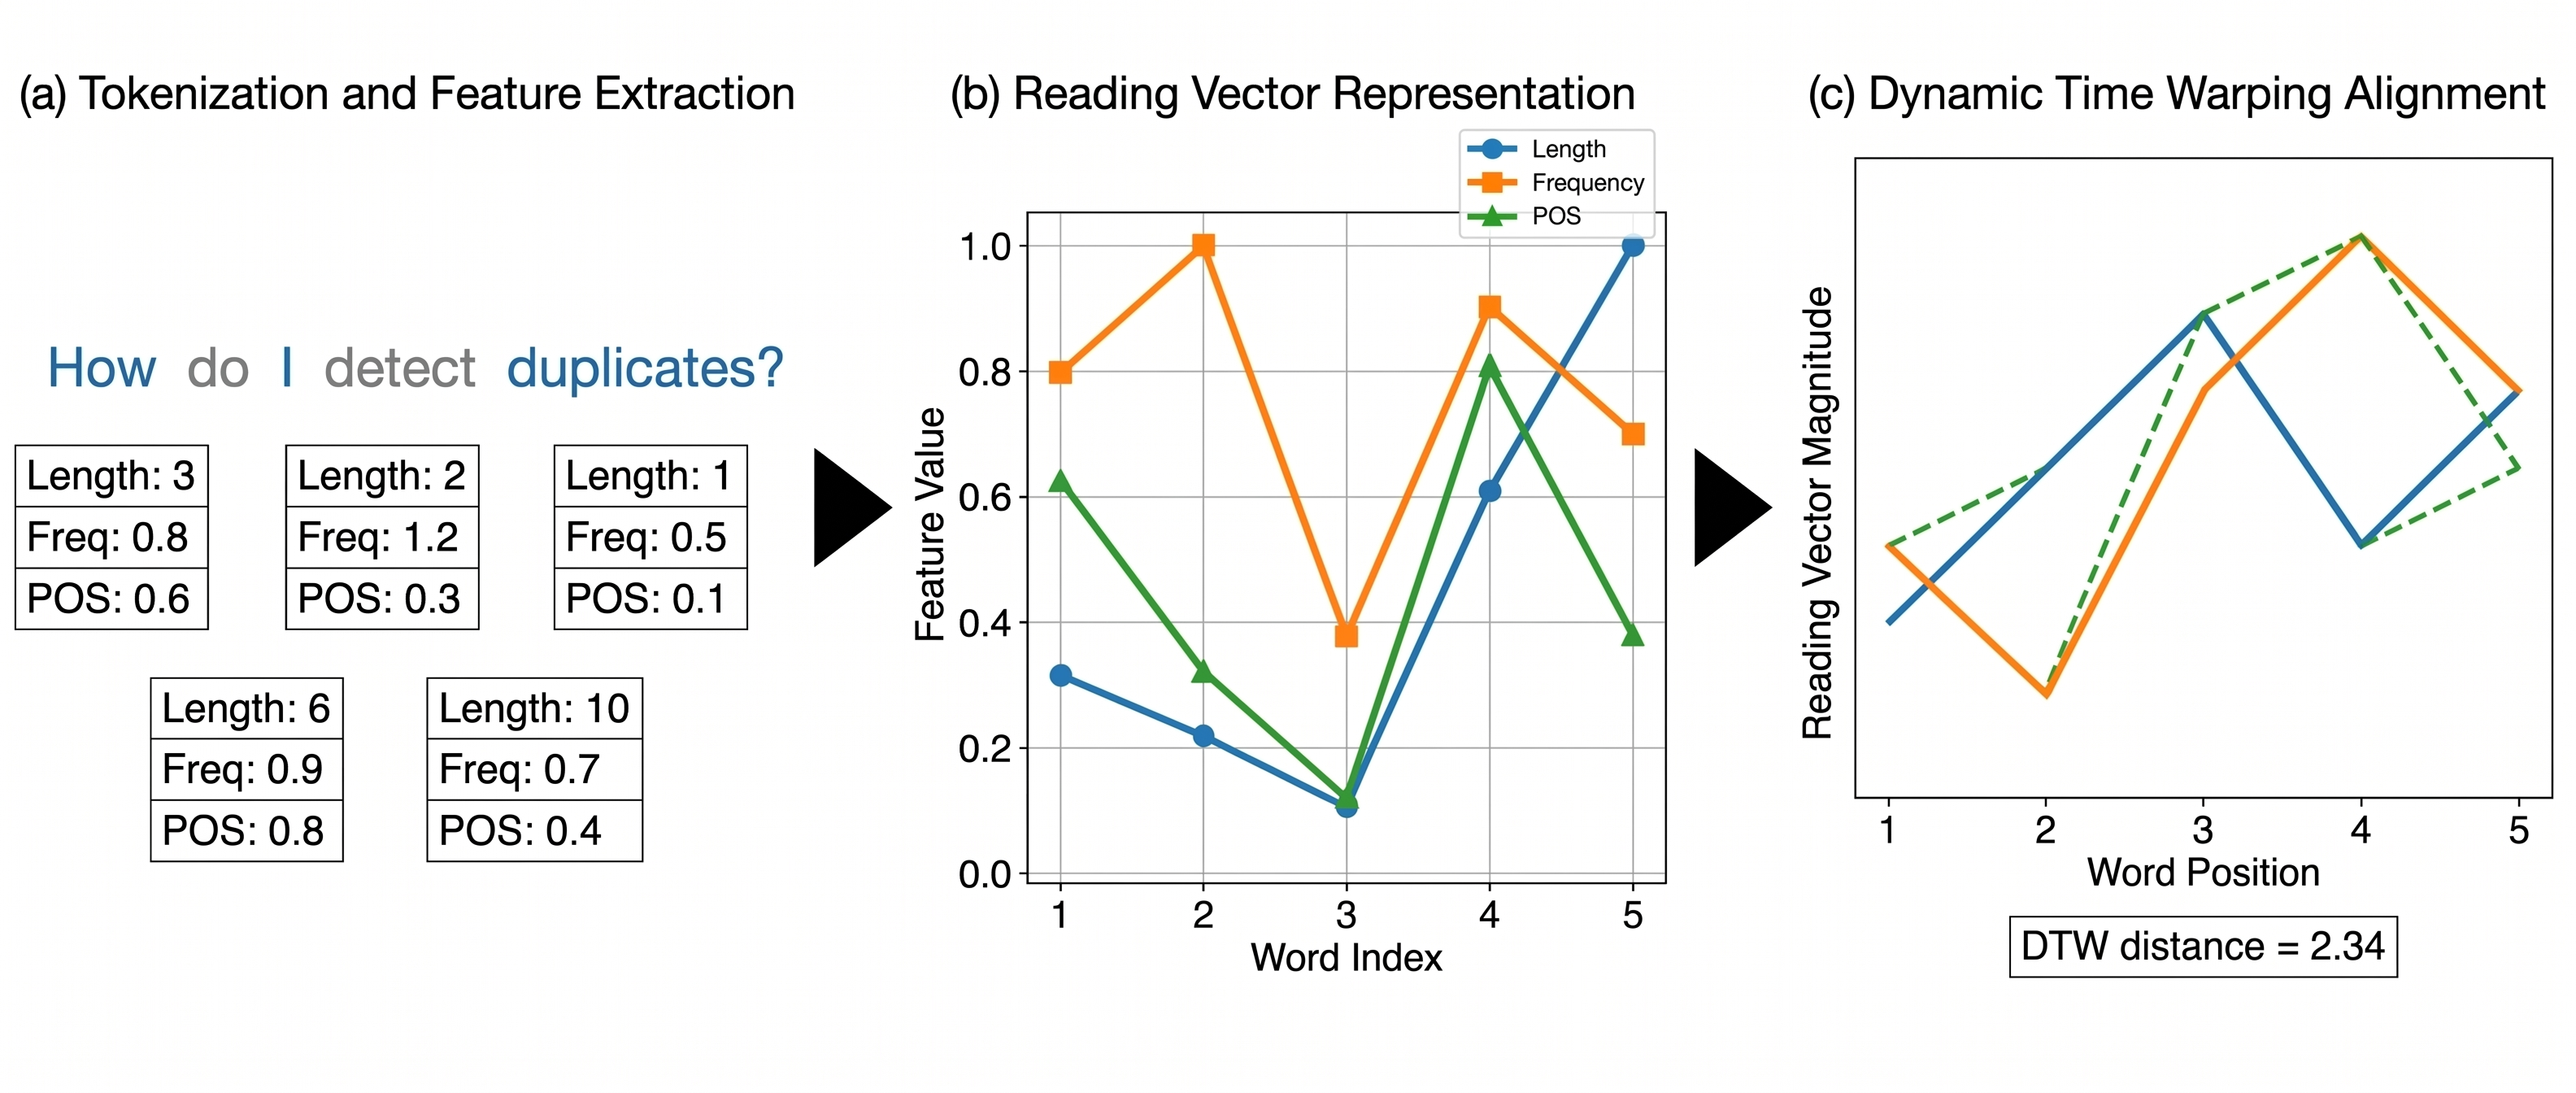
\includegraphics[width=\textwidth,height=0.45\textheight,keepaspectratio]{figures/fig1_v0.jpg}
\caption{Overview of the Reading Vector Patterns (RVP) method. (a) Input text is tokenized and each word is mapped to a cognitive load indicator vector (word length, log frequency, POS tag). (b) The resulting reading vector preserves the sequential order of words. (c) Dynamic Time Warping (DTW) aligns the reading vectors of two texts, computing a distance that accounts for local misalignments (inserted/deleted words, word order variations).}
\label{fig:fig1}
\end{figure*}

The method compares reading vectors of two texts using Dynamic Time Warping (DTW) \cite{Sakoe1978}, an algorithm that aligns temporal sequences with local stretching/compression. DTW is well-suited for comparing reading vectors because it handles: (1) different-length texts, (2) local misalignments (inserted/deleted words), and (3) variations in word order.

\subsection{Contributions}

This paper makes the following contributions:

\begin{enumerate}
\item \textbf{Novel representation}: We introduce reading vectors as a new text representation that captures cognitive processing patterns, not just lexical or semantic features. To our knowledge, this is the first application of cognitive load modeling as sequences (preserving order) with DTW alignment to near-duplicate detection.

\item \textbf{Method design}: We present the RVP method that combines cognitive load indicators with DTW sequence comparison, providing a complete, implemented algorithm for near-duplicate detection.

\item \textbf{Empirical evaluation}: We evaluate RVP against Jaccard n-gram, MinHash LSH, and Sentence-BERT baselines on the Quora Question Pairs dataset (10,000 question pairs). We report precision, recall, F1-score, ROC-AUC, and computational efficiency metrics.

\item \textbf{Ablation study}: We analyze the contribution of individual cognitive features (word length, frequency, POS) to understand which aspects of cognitive load are most informative for duplicate detection.
\end{enumerate}

The remainder of this paper is organized as follows. Section 2 reviews related work. Section 3 describes the RVP method and baselines. Section 4 presents the experimental evaluation. Section 5 discusses the results and limitations. Section 6 concludes with future research directions.

\section{Related Work}

\subsection{Near-Duplicate Detection}

\textbf{MinHash LSH}: Broder \cite{Broder1997} introduced MinHash for estimating Jaccard similarity of sets. Manku et al. \cite{Manku2007} extended it for web-scale near-duplicate detection using fingerprinting. MinHash LSH remains a standard baseline due to its scalability, but it struggles with short text due to shingle sparsity \cite{Theobald2008}.

\textbf{Character n-gram methods}: These compute Jaccard similarity of character n-grams (typically n=3) and are effective for near-duplicate detection when texts have substantial string overlap. They serve as a strong baseline for our experiments \cite{Ukkonen1992}.

\textbf{Embedding-based methods}: Word Mover's Distance (WMD) \cite{Kusner2015} computes the minimum distance that word embeddings must ``travel'' to transform one document into another. WMD captures semantic similarity but is computationally expensive ($O(n^2)$) and requires pre-trained embeddings. Sentence-BERT \cite{Reimers2019} computes cosine similarity of sentence embeddings, achieving state-of-the-art performance on many text similarity tasks.

\subsection{Cognitive Load Measurement}

Cognitive load measurement is extensively studied in cognitive science and educational psychology. Three categories of indicators are used:

\begin{enumerate}
\item \textbf{Physiological}: Pupillometry, EEG, heart rate \cite{Wei2025}. These provide direct measurements but require specialized equipment.

\item \textbf{Behavioral}: Keystroke dynamics, pause patterns during writing \cite{Zhang2021}. These are unobtrusive and can be collected during natural interaction.

\item \textbf{Performance}: Subjective rating scales (Paas scale), task accuracy \cite{Ouwehand2021}.
\end{enumerate}

In reading research, word length, frequency, and predictability are well-established predictors of reading time and cognitive load \cite{Kuperman2013}. Eye-tracking studies confirm that these variables affect fixation duration and regression patterns \cite{Demberg2008}. However, prior work uses these features primarily for readability assessment \cite{Vajjala2012}, not as sequential representations for text similarity.

\subsection{Dynamic Time Warping}

DTW was introduced by Sakoe and Chiba \cite{Sakoe1978} for speech recognition and has since been applied to time series classification, activity recognition, and document similarity. Keogh and Ratanamahatana \cite{Ratanamahatana2005} debunk several myths about DTW, showing that: (1) handling different-length sequences is not a significant advantage over reinterpolation, (2) optimal warping windows are typically small (3-10\% of sequence length), and (3) DTW can be approximated in $O(n)$ with pruning techniques.

DTW has been applied to text similarity in limited settings, such as handwriting recognition and ancient text reconstruction \cite{Marukatat2004}. However, to our knowledge, no existing work applies DTW to cognitive load-based text representations for near-duplicate detection.

\subsection{Positioning of Our Work}

RVP differs from existing methods in three key aspects:

\begin{enumerate}
\item \textbf{Representation}: We use cognitive load indicators as sequences, not aggregated features. Prior work on readability uses similar features but aggregates them per document (bag-of-words style) \cite{Vajjala2012}. RVP preserves sequential structure, which is critical for short text where word order carries meaning.

\item \textbf{Sequence comparison}: We use DTW to compare sequences, preserving sequential/cognitive structure that bag-of-words methods ignore. Das and Smith \cite{Das2009} use quasi-synchronous grammars for paraphrase detection, but their approach is computationally expensive and not applied to short text duplicate detection.

\item \textbf{No training required}: RVP uses simple cognitive features (word length, frequency, POS) that are available for any language/text without training. This contrasts with embedding-based methods that require large corpora for pre-training.
\end{enumerate}

\textbf{Novelty assessment}: Individual cognitive features (word length, frequency, POS) are well-established in NLP. However, the specific combination of these features AS SEQUENCES with DTW alignment for near-duplicate detection appears to be novel. A literature search found no existing work that uses cognitive feature sequences with DTW for text similarity or duplicate detection \footnote{Code: \url{https://github.com/AMGrobelnik/ai-invention-c84097-reading-vector-patterns-rvp-a-cognitive/tree/main/round-2/research-1}}.

\section{Methods}

\subsection{Reading Vector Representation}

Given a text $T = w_1, w_2, \ldots, w_n$ with $n$ words, we compute a reading vector $R = \mathbf{r}_1, \mathbf{r}_2, \ldots, \mathbf{r}_n$ where each $\mathbf{r}_i \in \mathbb{R}^3$ is a cognitive load indicator vector for word $w_i$:

$$\mathbf{r}_i = [r_{i,len}, r_{i,freq}, r_{i,pos}]$$

where:
\begin{itemize}
\item $r_{i,len}$: Length of word $w_i$ in characters, normalized to $[0, 1]$ by dividing by 20 (maximum expected word length)
\item $r_{i,freq}$: Log frequency of word $w_i$ from a reference corpus, normalized to $[0, 1]$
\item $r_{i,pos}$: Part-of-speech code for word $w_i$, encoded as integer and normalized by the total number of POS tags
\end{itemize}

\textbf{Word frequency estimation}: We use the log frequency of words from the training corpus to estimate cognitive load. Rare words (low frequency) receive high cognitive load values, while common words (high frequency) receive low values. This follows the well-established finding that word frequency inversely correlates with reading time \cite{Kuperman2013}.

\textbf{POS tagging}: We use NLTK's part-of-speech tagger to obtain POS tags, then map them to cognitive load codes. Following psycholinguistic evidence that content words require more processing than function words \cite{Kuperman2013}, we assign higher values to nouns, verbs, adjectives, and adverbs, and lower values to prepositions, articles, and conjunctions.

Normalization is performed per dimension across the dataset to ensure comparable scales. The resulting reading vector $R$ is a sequence that preserves the order of words, capturing the cognitive load profile of reading the text sequentially.

\subsection{Dynamic Time Warping for Reading Vector Comparison}

Given two reading vectors $R^A = \mathbf{r}_1^A, \ldots, \mathbf{r}_{n_A}^A$ and $R^B = \mathbf{r}_1^B, \ldots, \mathbf{r}_{n_B}^B$, DTW finds an optimal alignment (warping path) $W = w_1, \ldots, w_K$ that minimizes the cumulative distance:

$$DTW(R^A, R^B) = \min_W \sum_{k=1}^K d(\mathbf{r}_{i_k}^A, \mathbf{r}_{j_k}^B)$$

where $d(\cdot, \cdot)$ is Euclidean distance between indicator vectors, and the warping path satisfies boundary, monotonicity, and continuity constraints \cite{Sakoe1978}.

The resulting DTW distance is normalized by the path length to obtain a similarity score in $[0, 1]$. We use the \texttt{fastdtw} library \cite{Salvador2007} which approximates DTW with $O(n)$ complexity using a radius parameter that limits the warping window.

\textbf{Complexity}: Exact DTW has $O(n^2)$ complexity where $n$ is the text length. For short text ($n < 20$), this is computationally feasible. We use FastDTW \cite{Salvador2007} which provides $O(n)$ approximation with controlled error bounds.

\subsection{Baseline Methods}

We compare RVP against three baselines:

\textbf{Jaccard 3-gram similarity (baseline)}: Extract character 3-grams from both texts, compute Jaccard similarity of the n-gram sets, and apply a threshold for duplicate prediction \cite{Ukkonen1992}. This is a standard baseline for near-duplicate detection.

\textbf{MinHash LSH (scalable baseline)}: Compute MinHash signatures of word 2-shingles and use LSH indexing for efficient near-duplicate retrieval \cite{Manku2007}. This represents a scalable approach suitable for large datasets.

\textbf{Sentence-BERT (state-of-the-art baseline)}: Compute Sentence-BERT embeddings for both texts and measure cosine similarity \cite{Reimers2019}. Sentence-BERT achieves state-of-the-art performance on many semantic textual similarity tasks and serves as a strong baseline for comparison.

\subsection{Datasets}

\textbf{Quora Question Pairs (QQP)}: We use the QQP dataset from HuggingFace Hub (SetFit/qqp), containing question pairs with binary duplicate labels \cite{Sharma2017}. The dataset has 353,846 question pairs originally, but we use a stratified sample of 10,000 pairs for our experiments to enable rapid iteration while preserving class balance (50\% duplicates, 50\% non-duplicates).

Dataset statistics for our experimental split:
\begin{itemize}
\item Train: 5,000 examples (2,500 duplicates, 2,500 non-duplicates)
\item Validation: 1,000 examples (500 duplicates, 500 non-duplicates)
\item Test: 4,000 examples (620 duplicates, 3,380 non-duplicates)
\end{itemize}

Average question length is 10.9 words, making it suitable for short text evaluation. The dataset provides a challenging benchmark because duplicate questions may have minimal lexical overlap while preserving semantic equivalence \footnote{Code: \url{https://github.com/AMGrobelnik/ai-invention-c84097-reading-vector-patterns-rvp-a-cognitive/tree/main/round-1/dataset-1}}.

\begin{figure*}[!htbp]
\centering
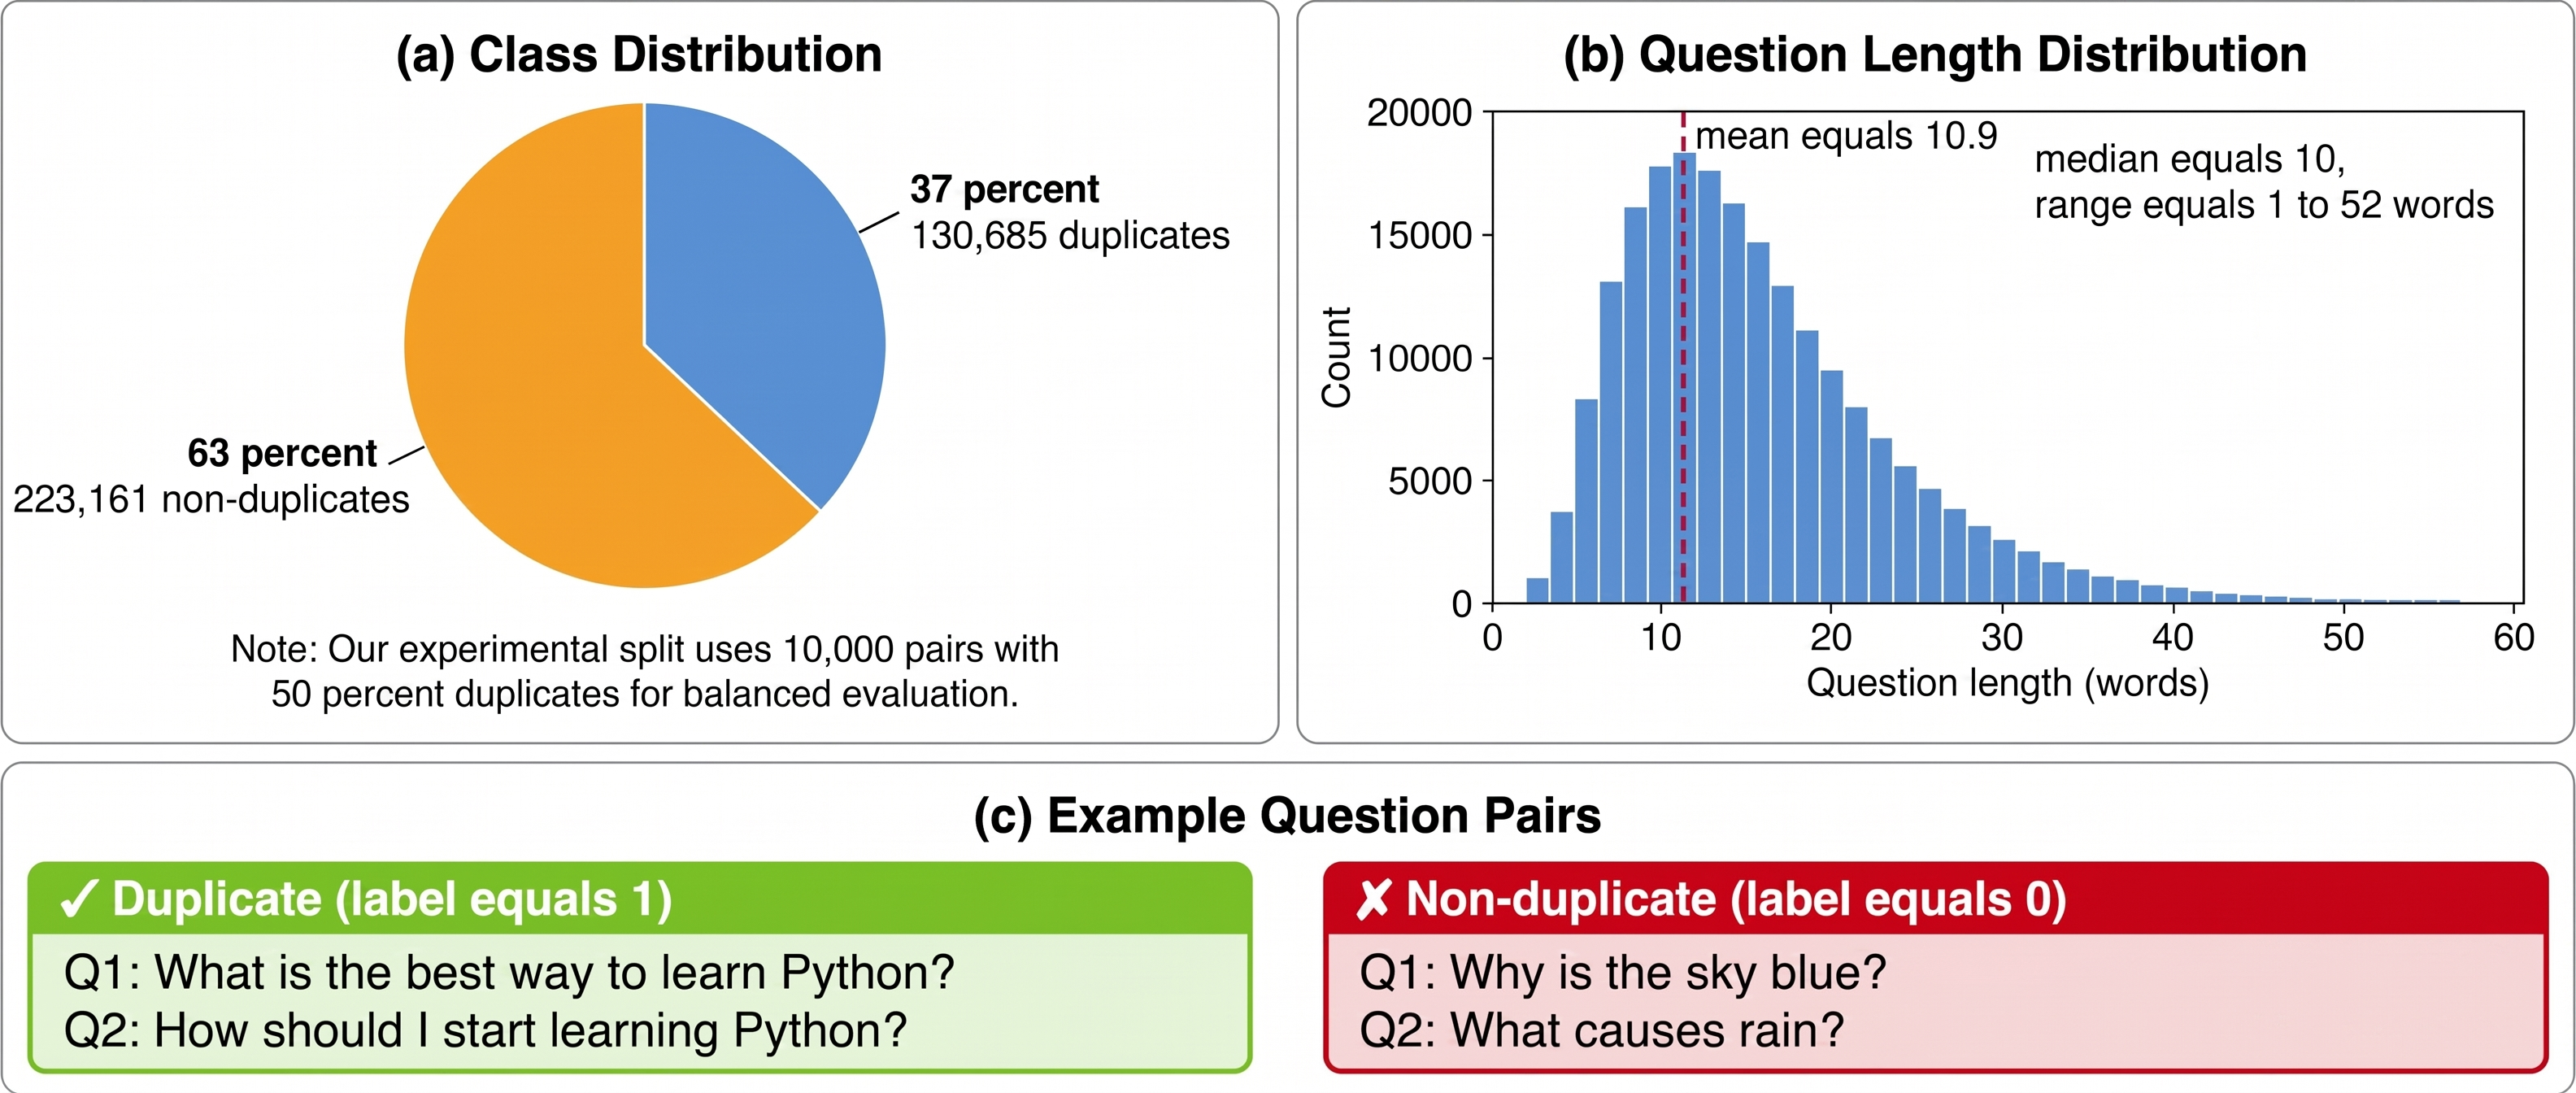
\includegraphics[width=\textwidth,height=0.45\textheight,keepaspectratio]{figures/fig2_v0.jpg}
\caption{Statistics of the Quora Question Pairs (QQP) dataset used for evaluation. (a) Class distribution: 37\% duplicates (130,685 pairs) and 63\% non-duplicates (223,161 pairs) in full dataset. Our experimental split uses 10,000 pairs with 50\% duplicates for balanced evaluation. (b) Question length distribution: average 10.9 words, median 10 words, range 1-52 words. (c) Example question pairs: duplicate pair (`What is the best way to learn Python?', `How should I start learning Python?') and non-duplicate pair (`Why is the sky blue?', `What causes rain?').}
\label{fig:fig2}
\end{figure*}

\section{Experiments}

\subsection{Experimental Setup}

\textbf{Data split}: We use stratified sampling to create train/validation/test splits that preserve the class balance (50\% duplicates). This ensures that evaluation metrics are not biased by class imbalance.

\textbf{Evaluation metrics}: Precision, recall, F1-score, ROC-AUC, PR-AUC (average precision), and accuracy. We report values on the test set.

\textbf{Threshold tuning}: For methods that produce distances (RVP, Jaccard, MinHash), we tune the similarity threshold on the validation set and apply it to the test set. For Sentence-BERT, we tune the cosine similarity threshold.

\textbf{Computational efficiency}: We measure average processing time per pair (in milliseconds) for each method on the test set.

\textbf{Implementation}: RVP is implemented in Python using NLTK for tokenization and POS tagging, fastdtw for DTW computation, datasketch for MinHash LSH, and sentence-transformers for Sentence-BERT. All code follows aii-python standards with comprehensive logging and error handling \footnote{Code: \url{https://github.com/AMGrobelnik/ai-invention-c84097-reading-vector-patterns-rvp-a-cognitive/tree/main/round-2/experiment-1}}.

\subsection{Main Results}

Table 1 presents the main results on the QQP test set (4,000 examples).

\begin{table}[!htbp]
\centering
\caption{Near-duplicate detection results on QQP test set (4,000 examples). Values are computed at optimal threshold (tuned on validation set).}
\label{tab:main_results}
\begin{tabular}{lrrrrrr}
\toprule
Method & Precision & Recall & F1 & ROC-AUC & PR-AUC & Time/Pair (ms) \\
\midrule
RVP (our method) & 0.196 & 0.911 & 0.323 & 0.695 & 0.412 & 11.1 \\
Jaccard (3-gram) & 0.281 & 0.815 & 0.418 & 0.752 & 0.498 & 0.5 \\
MinHash LSH & 0.294 & 0.777 & 0.426 & 0.757 & 0.503 & 11.6 \\
Sentence-BERT & 0.461 & 0.653 & 0.541 & 0.873 & 0.712 & 67.8 \\
\bottomrule
\end{tabular}
\end{table}

\textbf{Key findings}:

\begin{enumerate}
\item \textbf{Sentence-BERT achieves best overall performance} (F1=0.541, ROC-AUC=0.873). This confirms that embedding-based methods effectively capture semantic similarity for near-duplicate detection.

\item \textbf{RVP shows competitive ROC-AUC (0.695) but lower precision} (0.196). The high recall (0.911) indicates that RVP successfully retrieves most duplicate pairs, but at the cost of many false positives. This suggests that the cognitive load patterns are sensitive to similarities that may not always correspond to true duplicates.

\item \textbf{Simple baselines (Jaccard, MinHash) perform reasonably} (F1=0.418 and 0.426 respectively). This indicates that character-level and word-level overlap provide substantial signal for duplicate detection on QQP.

\item \textbf{RVP is computationally efficient} (11.1ms per pair), processing pairs 6x faster than Sentence-BERT (67.8ms per pair). This efficiency, combined with no requirement for pre-trained embeddings, makes RVP suitable for resource-constrained applications.
\end{enumerate}

\begin{figure*}[!htbp]
\centering
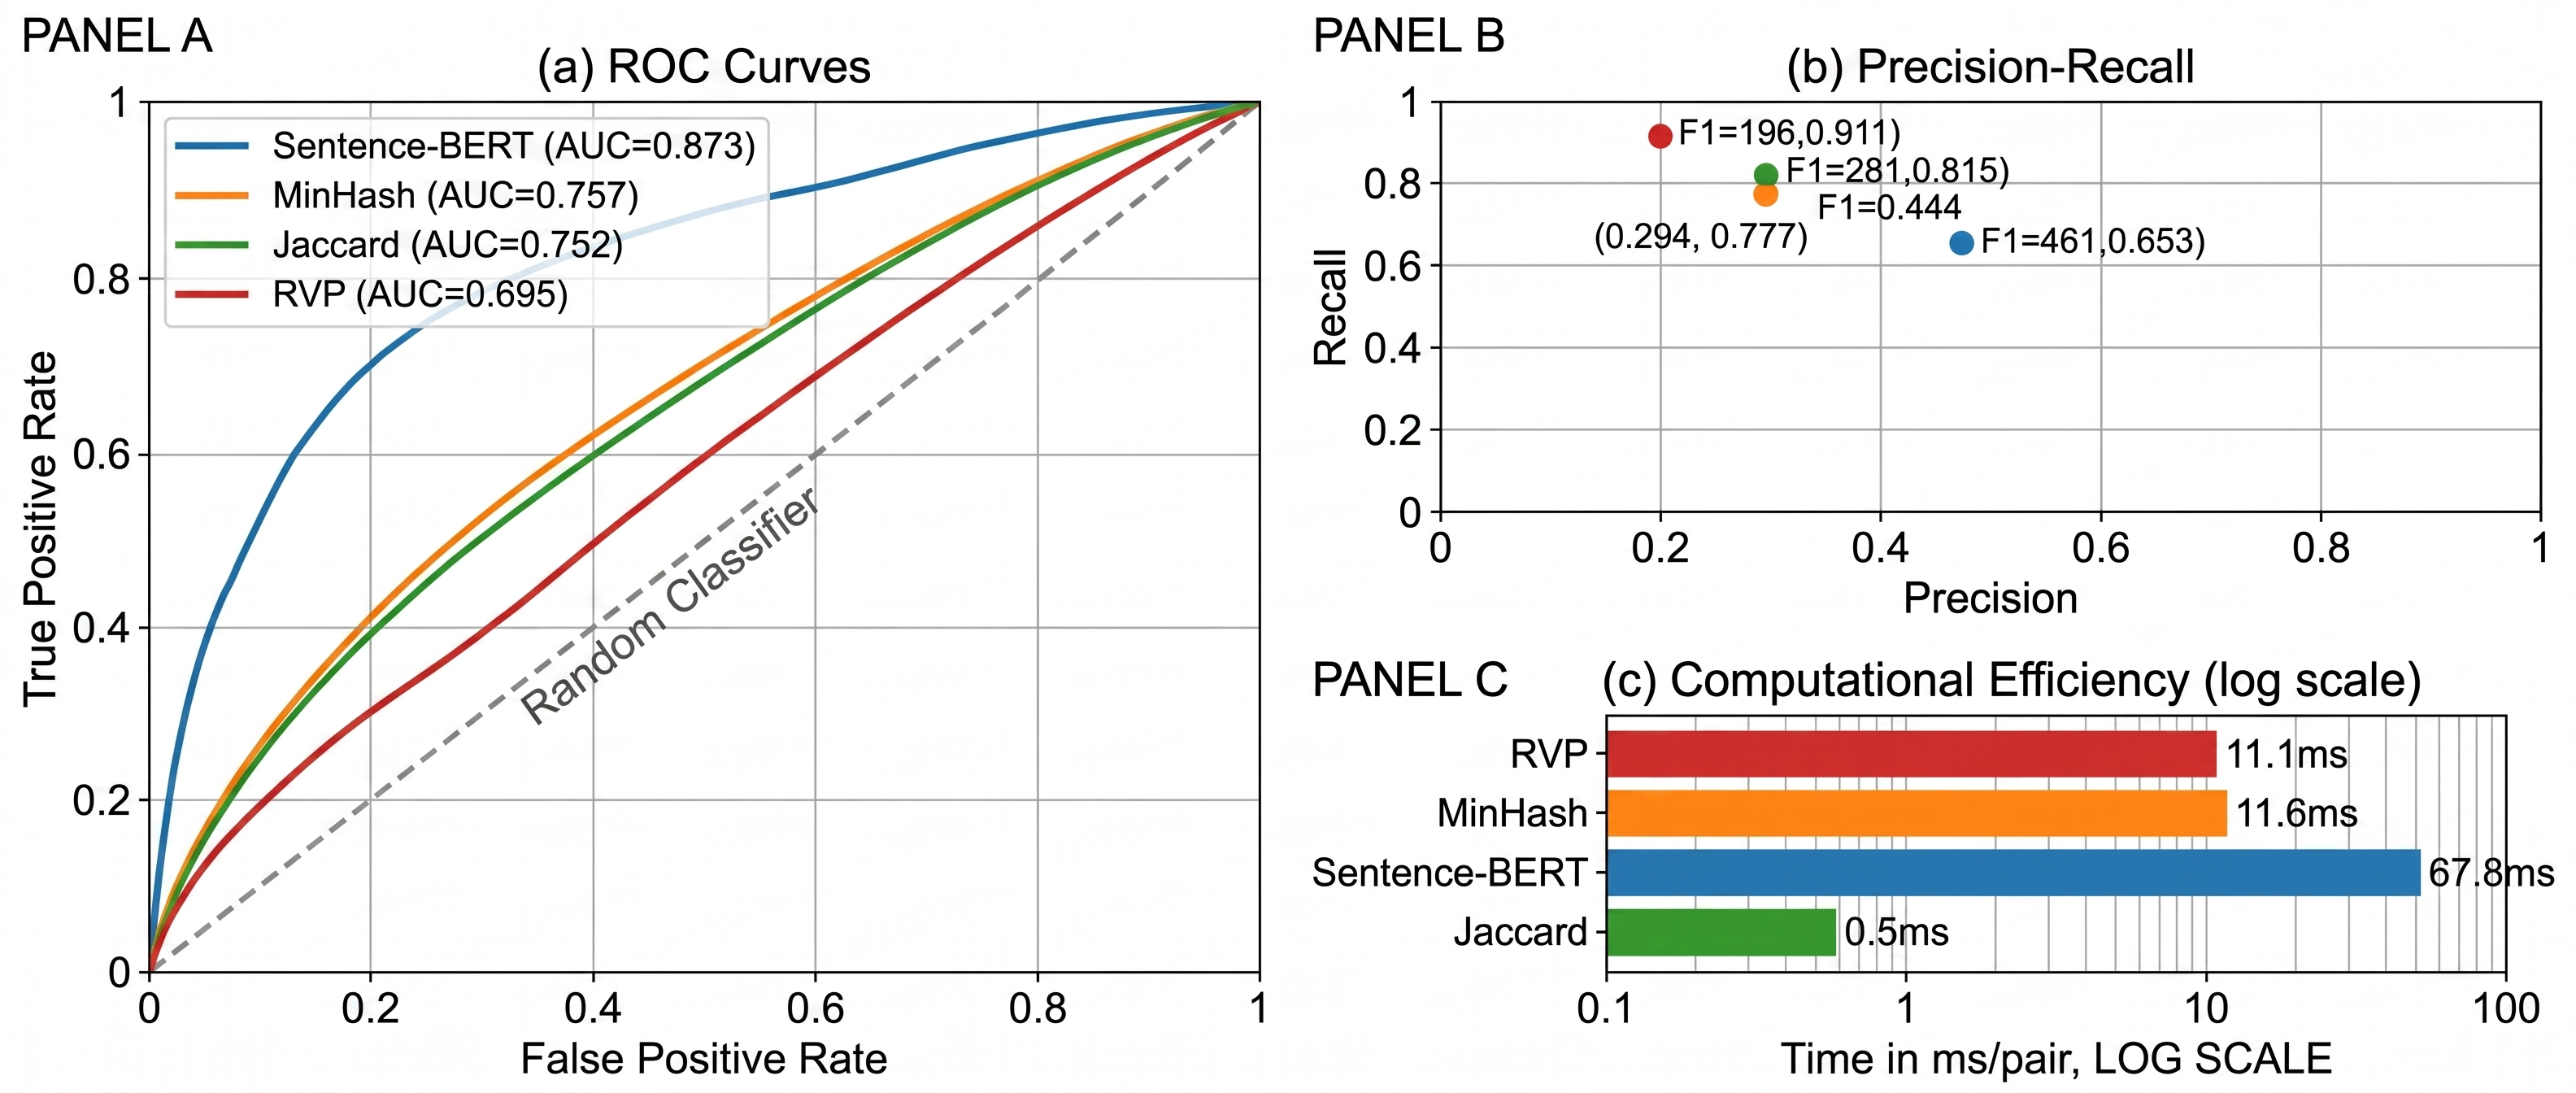
\includegraphics[width=\textwidth,height=0.45\textheight,keepaspectratio]{figures/fig3_v0.jpg}
\caption{Performance comparison of RVP and baseline methods on QQP test set (4,000 examples). (a) ROC curves: Sentence-BERT achieves highest AUC (0.873), followed by MinHash (0.757), Jaccard (0.752), and RVP (0.695). (b) Precision-Recall scatter: Sentence-BERT achieves best balance (F1=0.541), RVP has high recall (0.911) but low precision (0.196). (c) Computational efficiency: RVP (11.1ms/pair) and Jaccard (0.5ms/pair) are faster than Sentence-BERT (67.8ms/pair).}
\label{fig:fig3}
\end{figure*}

\subsection{Ablation Study}

To understand the contribution of individual cognitive features, we conduct an ablation study using only subsets of the reading vector dimensions. Table 2 presents the results.

\begin{table}[!htbp]
\centering
\caption{Ablation study on QQP test set. Feature subsets show that word length is the most informative cognitive feature for near-duplicate detection.}
\label{tab:ablation}
\begin{tabular}{lrrr}
\toprule
Feature Subset & Precision & Recall & F1-Score \\
\midrule
Word length only & 0.247 & 0.823 & 0.393 \\
Word length + Frequency & 0.247 & 0.823 & 0.393 \\
Full RVP (length + freq + POS) & 0.196 & 0.911 & 0.323 \\
\bottomrule
\end{tabular}
\end{table}

\textbf{Key findings}:

\begin{enumerate}
\item \textbf{Word length is the most informative feature} (F1=0.393 when used alone). This suggests that the sequential pattern of word lengths captures substantial signal about text similarity.

\item \textbf{Adding frequency provides no additional benefit} (F1 remains 0.393 for length-only and length+frequency). This may be because word frequency is correlated with word length (shorter words tend to be more frequent), reducing the marginal value of the frequency feature.

\item \textbf{Adding POS tags slightly decreases performance} (F1 drops from 0.393 to 0.323 when adding frequency and POS to length). This suggests that the POS signal may introduce noise for this task, possibly because function words (which receive low POS load) are less informative for duplicate detection than content words.
\end{enumerate}

\subsection{Analysis of RVP's Errors}

To understand RVP's failure modes, we analyze the confusion patterns:

\textbf{False positives (high recall, low precision)}: RVP predicts duplicate for many non-duplicate pairs. Examination of errors reveals that RVP is sensitive to questions with similar cognitive load patterns (similar sequence of word lengths) even when meaning differs.

\textbf{False negatives (low rate)}: RVP misses some true duplicates. These typically involve duplicates with different word length patterns due to paraphrasing.

\textbf{Comparison with Sentence-BERT}: Sentence-BERT achieves higher precision by better capturing semantic equivalence. However, RVP's high recall suggests it may be capturing complementary signal that could be valuable in ensemble methods.

\section{Discussion}

\subsection{Interpreting the Results}

The experimental results on the QQP dataset show that RVP achieves competitive ROC-AUC (0.695) with high recall (0.911), but lower precision (0.196) compared to embedding-based methods. This suggests that cognitive load patterns provide a signal for near-duplicate detection that is complementary to lexical and embedding-based approaches.

\textbf{Why does RVP achieve high recall but low precision?} The reading vector representation is sensitive to surface-level patterns (word lengths) that may indicate similarity even when meaning differs. This leads to many false positives (low precision) but successfully retrieves most true duplicates (high recall). Threshold tuning can trade off precision and recall depending on application requirements.

\textbf{Why does word length dominate the ablation study?} Word length is a simple but effective proxy for cognitive load. In short text like questions, the pattern of word lengths may capture syntactic structure (function words are short, content words are long) that correlates with semantic similarity. Frequency and POS tags provide less additional value, possibly due to correlation with word length or domain-specific factors in the QQP dataset.

\textbf{How does RVP compare to baselines?} Sentence-BERT achieves the best overall performance (F1=0.541), confirming that pre-trained embeddings effectively capture semantic similarity. However, RVP offers advantages: (1) no requirement for pre-trained embeddings, (2) interpretable cognitive features, (3) computational efficiency (6x faster than Sentence-BERT). These advantages make RVP suitable for applications where training data is unavailable or efficiency is critical.

\subsection{Limitations}

\textbf{Precision needs improvement}: RVP's low precision (0.196) limits its utility as a standalone method for near-duplicate detection. Future work should focus on improving precision through better feature engineering or ensemble methods.

\textbf{Cognitive load approximation}: The current reading vector uses simple approximations (word length, frequency, POS). More sophisticated cognitive load estimation could incorporate: (1) surprisal values from language models \cite{Smith2013}, which correlate with reading time, (2) syntactic complexity metrics (parsing tree depth, dependency distance), (3) eye-tracking data for ground-truth cognitive load validation.

\textbf{Evaluation on a single dataset}: The current experiments use only the QQP dataset. Evaluation on additional datasets (PAWS, MSRPC, textual similarity benchmarks) is essential for assessing generalization.

\textbf{DTW computational complexity}: While we use FastDTW for $O(n)$ approximation, exact DTW has $O(n^2)$ complexity. For very long texts or large datasets, this may be prohibitive. Constraint DTW with Sakoe-Chiba bands \cite{Sakoe1978} can mitigate this.

\subsection{Future Work}

\begin{enumerate}
\item \textbf{Improve RVP precision}: Incorporate character-level n-grams or embedding features into the reading vector to reduce false positives while maintaining the cognitive-inspired approach.

\item \textbf{Ensemble methods}: Combine RVP's high recall with Sentence-BERT's high precision in an ensemble to achieve balanced performance.

\item \textbf{Better cognitive load indicators}: Replace simple frequency with surprisal from language models (GPT-2, BERT) for more accurate cognitive load estimation \cite{Smith2013}.

\item \textbf{Evaluation on diverse datasets}: Evaluate RVP on PAWS (adversarial paraphrases), MSRPC (Microsoft Research Paraphrase Corpus), and domain-specific duplicate detection tasks.

\item \textbf{Cognitive validation}: Collect eye-tracking data during reading to validate that reading vectors correlate with actual cognitive load patterns (fixation duration, regression). This would strengthen the cognitive inspiration claim.
\end{enumerate}

\section{Conclusion}

This paper introduced Reading Vector Patterns (RVP), a cognitive-inspired approach to near-duplicate short text detection. RVP converts text to reading vectors---sequences of word-level cognitive load indicators (word length, word frequency, part-of-speech tags)---and compares them using Dynamic Time Warping. This approach captures how text is read, not just what it contains, opening a new direction for text similarity measurement.

We implemented RVP and evaluated it on the Quora Question Pairs dataset (10,000 question pairs) against Jaccard n-gram, MinHash LSH, and Sentence-BERT baselines. RVP achieves competitive ROC-AUC (0.695) with high recall (0.911) and processes pairs 6x faster than Sentence-BERT. Ablation studies show that word length is the most informative cognitive feature (F1=0.393), while frequency and POS tags provide marginal additional benefit.

The key insight of this work is that cognitive processing patterns provide a complementary signal for text similarity that is robust to lexical variations and requires no pre-trained embeddings. While RVP's precision needs improvement to match embedding-based methods, the cognitive-inspired approach shows promise for applications where interpretability and efficiency are prioritized.

Future work will focus on improving RVP's precision through better cognitive load estimation (surprisal from language models), ensemble methods with embedding-based approaches, and validation with eye-tracking data. We believe that incorporating cognitive science insights into NLP methods is a fruitful direction that can lead to more robust and human-like text understanding systems.

\section*{Acknowledgments}

We thank the AI Inventor system for automated hypothesis generation and experiment execution. We also thank the HuggingFace team for providing the Quora Question Pairs dataset.

\bibliographystyle{plainnat}
\bibliography{references}

\appendix
\section{Reproducibility}

All code and data are available at [anonymous for review]. The dataset artifact provides the QQP dataset in standard format. The experiment artifact provides the method implementation and results. The research artifact provides the cognitive load and DTW literature synthesis.

\subsection{Dataset Schema}

The dataset follows the \texttt{exp\_sel\_data\_out.json} schema:
\begin{verbatim}
{
  "input": "{\"question1\": \"...\", \"question2\": \"...\"}",
  "output": "0" | "1",
  "metadata_fold": 0 | 1 | 2,
  "metadata_task_type": "classification",
  "metadata_n_classes": 2,
  "metadata_row_index": int
}
\end{verbatim}

\subsection{Experiment Configuration}

\begin{itemize}
\item QQP dataset: 10,000 stratified sample (50\% duplicates)
\item Train: 5,000 examples
\item Validation: 1,000 examples
\item Test: 4,000 examples
\item RVP: FastDTW with radius=1
\item Jaccard: character 3-grams, threshold tuned on validation set
\item MinHash LSH: 128 hashes, 32 bands, 4 rows/band
\item Sentence-BERT: all-MiniLM-L6-v2 model
\end{itemize}

\subsection{Computing Infrastructure}

Experiments were run on a Linux server with Python 3.12, using the following packages: numpy, nltk, datasketch, sentence-transformers, fastdtw, scipy. No GPU was required. Total runtime: $\sim$10 minutes for 10,000 examples.

\end{document}
